    \begin{lemma}[О барицентрическом подразбиении]\label{BaricentrLemma}
        Пусть $f\colon T^q \to X$~--- сингулярный симплекс. Тогда его барицентрическое поразбиение~--- это
        \[ \beta\colon C_{q}(X) \to C_{q}(X), \quad  \beta f = \sum_{\tau \in S_{q + 1}}\sign(\tau) f_{\tau}, \]
        где $f_{\tau}$ определяется следующим образом: исходный симплекс $T^{q}$ мы можем барицентрически подразбить на симплексы $T'_{q} = \{ x \ \vert \ x_{\tau(0)} \le x_{\tau(1)} \le \ldots \le x_{\tau(q)}\}$,
        в которых вершины нумеруются согласно размерностям граней. Тогда мы полагаем  $f_{\tau} \eqdef f\vert_{T'_{q}}$.

        Тогда $\partial \beta = \beta \partial$ и  $\beta_{*}([\alpha]) = [\alpha] \ \forall [\alpha] \in H_{q}(X)$. Иными словами,
        барицентрическое подразбиение не влияет на гомологический класс.
    \end{lemma}

    \begin{proof}
        Для первого утверждения достаточно проверить, что в сумме все внутренние грани встречаются с противоположным знаком, это ясно из картинки.
        Первое утверждение даёт нам, что $\beta \in \Hom_{\fC\fh}(C_{\bullet}, C_{\bullet})$.

        Для доказательства второго утверждения мы построим цепную гомотопию $D\colon C_{q}(X) \to C_{q + 1}(X)$ между $\beta$ и постоянным отображением.

        Пусть $f\colon T^{q} \to X$, тогда $D(f)$ определяется следующим образом:
        барицентрически разобьем призму $I \times T^{q}$ на симплексы и рассмотрим проекцию
        \[ p\colon I \times T^q \to T^q. \]
        Тогда $D(f)$~--- это $(q + 1)$-мерный сингулярный симплекс, являющийся суммой композиций $f$ и проекции $p$, суженной на симплексы в разбиении $I \times T^{q}$.
        \begin{center}
            \textcolor{magenta}{можно нарисовать картинку для отрезка, в принципе.}
        \end{center}

        Из того, как устроена нумерация в барицентрическом разбиении призмы, нетрудно видеть, что $D$~--- гомотопия между $\beta$ и $\mathrm{id}$,
        то есть
        \[ f - \beta(f) = D \partial(f) + \partial D(f).  \]
        \textcolor{ForestGreen}{Чтоб понять всё это, надо опять позалипать на эту картиночку с призмой, как в теореме~\ref{HomotopyImpliesHomotopy}.}\footnote{Возможно, всё это место стоит строго формально переписать из Хачтера.}
    \end{proof}

    Следующая лемма говорит нам, что для вычисления сингулярных гомологий достаточно рассматривать лишь \emph{маленькие} сингулярные симплексы.
    В случае симплициальных гомологий это можно было бы формулировать в терминах диаметров, а в случае сингулярных мы будем говорить об этом
    в терминах покрытий.

    \begin{lemma}[Об измельчении]\label{IzmelchLemma}
        Пусть $\cU = \{ U_{\alpha} \}$~--- конечное открытое покрытие $X$.
        Пусть $C_{q}^{\cU}(X)$ порождено сингулярными симплексами $f \in C_{q}(X)$ такими, что $\exists \alpha\colon f(T_{q})  \subset U_{\alpha}$.

        Тогда вложение $i\colon C^{\cU}_{q}(X) \xrightarrow{i} C_{q}(X)$ индуцирует изоморфизм групп гомологий
        $H_{\bullet}(X) \cong H_{\bullet}^{\cU}(X)$.
    \end{lemma}
    \begin{proof}
        Заметим, что для достаточно большого $n$ по лемме Лебега $c \in C_{q}(X) \Rightarrow \beta^n(c) \in C_{q}^{\cU}(X)$.
        Кроме того, по лемме~\ref{BaricentrLemma} $c$ и $\beta^n(c)$ гомологичны (то есть, представляют один м тот же класс гомологий).
        Это даёт нам, что любой гомологический класс мз $H_{q}(C_{\bullet})$ имеет представителя в $C_{q}^{\cU}(X)$, то есть, что
        отображение $H^{\cU}_{q}(X) \to H_{q}(X)$ сюръективно.


        Кроме того, также по лемме~\ref{BaricentrLemma}, если $c$~--- цикл из $C_{q}^{\cU}$, то
        $c - \beta^n(c)$~--- граница цепи из $C_{q + 1}^{U}$, так как
        \[ c - \beta^n(c) =\underbrace{D\partial c}_{ = 0, \text{ так как $c$~--- цикл}} - \partial D c = \partial(-Dc) \in B_{q}\lr*{C_{q}^{\cU}(X)}.\]

        С другой стороны, так как $c$ и $\beta^n(c)$ гомологичны, их разность~--- граница (элемент $B_{q}(C_{q}(X))$).
        Таким образом, если цепь из $C_{q}^{\cU}$ лежит в $B_{q}\lr*{C_{q}(X)}$, то она лежит и в $B_{q}\lr*{C_{q}^{\cU}(X)}$.
        Это даёт нам инъективность отображения $H^{\cU}_{q}(X) \to H_{q}(X)$.
    \end{proof}

    \begin{remark}
       Заметим, что построенные в доказательстве отображения переводят цепи в $A$ в цепи в $A$, а значит, выдерживают факторизацию по $A$.
       Этот факт даёт нам версию леммы об измельчении для относительных гомологий, которым мы и будем пользоваться.
    \end{remark}

    Обзаведемся еще одним полезным фактом:
    Посмотрим на такой факт из гомологической алгебры:

    \begin{lemma}[5-лемма]\label{5-lemma}
        Рассмотрим диаграмму
        \begin{center}
            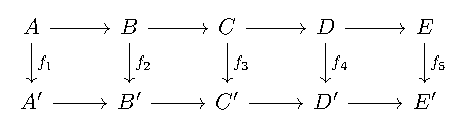
\includegraphics{lectures/0/pictures/cd_7}
        \end{center}
        в которой строки точны, $f_2, f_4$~--- изоморфизмы, $f_1$~--- эпиморфизм, $f_5$~--- мономорфизм.
        Тогда $f_3$~--- изоморфизм.
    \end{lemma}
    \begin{proof}
        Есть в любом курсе гомологической алгебры.
    \end{proof}

    Из неё немедленно следует следующий простой факт:

    \begin{lemma}\label{HomotopyEquivalencePair}
        Если пара $(X, A)$ гомотопически эквивалентна паре $(Y, B)$, то $H_{\bullet}(X, A) = H_{\bullet}(Y, B)$.
    \end{lemma}
    \begin{proof}
        Запишем длинную точную последовательность для обоих пар:
        \begin{center}
            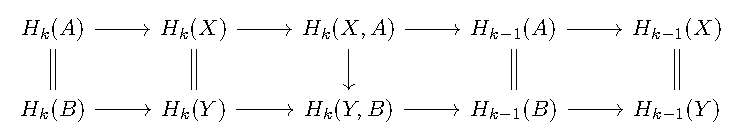
\includegraphics{lectures/0/pictures/cd_8}
        \end{center}
        Тогда всё следует из 5-леммы~\ref{5-lemma}
    \end{proof}

    Наконец, мы можем доказать интересующую нас теорему:

    \begin{theorem}\label{FactorizationTheorem}
        В общем случае отображение $X \to X \cup CA$ индуцирует изоморфизм
        \[ H_{q}(X, A) \to H_{q}(X \cup CA, CA) = H_{q}(X \cup CA, a) = \widetilde{H}_{q}(X \cup CA), \]
        где $a$~--- вершина конуса.

        Если $(X, A)$~--- пара Борсука, то отображение проекции $p\colon X \to X/A, \ A \mapsto a$ индуцирует изоморфизм
        \[ H_{q}(X, A) \xrightarrow{p_{*}} H_{q}(X/A, a) = \widetilde{H}_{q}(X/A). \]
    \end{theorem}

    \begin{proof}
        Рассмотрим открытое покрытие $X \cup CA$ вида:
        \[ X \cup CA \subset ((X \cup CA)\setminus X) \cup (X \cup \overline{C}A), \quad \cU \eqdef \{ (X \cup CA)\setminus X, (X \cup \overline{C}A) \} \]
        где $\overline{C}A$~--- нижняя открытая половина конуса $CA$.

        По лемме~\ref{IzmelchLemma} об измельчении мы вместо $H_{q}(X \cup CA, CA)$ можем рассматривать $H_{q}^{\cU}(X \cup CA, CA)$.

        А теперь, заметим, что по тому, как мы взяли покрытие,
        \[ C_{q}^{\cU}(X \cup CA, CA) = C_{q}^{\cU}(X \cup CA)/C_{q}^{\cU}(CA) = C_{q}\lr*{X \cup \overline{C}A}/C_{q}\lr*{\overline{C}A} = C_{q}\lr*{X \cup \overline{C}A, \overline{C}A}. \]

        А значит, из гомотопической эквивалентности и леммы~\ref{HomotopyEquivalencePair} мы имеем
        \[ H_{q}(X \cup CA, CA) = H_{q}(X \cup \overline{C}A, \overline{C}A) = H_{q}(X, A). \]

        Вторая часть первого равенства из условия теоремы следует из следствия~\ref{ParaCor1}.

        Пусть теперь (X, A)~--- пара Борсука. Тогда по утверждению~\ref{BorsukPairProp} $X \cup CA \sim X/A$, а значит,
        $H_{q}(X, A) \cong \widetilde{H}_{q}(X/A)$.
    \end{proof}
